\documentclass[dvipdfmx]{jarticle}
\usepackage{graphicx}
\usepackage{url}
\usepackage[top=30truemm,bottom=30truemm,left=25truemm,right=25truemm]{geometry}
\usepackage{listings,jvlisting}

\lstset{
  basicstyle={\ttfamily},
  identifierstyle={\small},
  commentstyle={\smallitshape},
  keywordstyle={\small\bfseries},
  ndkeywordstyle={\small},
  stringstyle={\small\ttfamily},
  frame={tb},
  breaklines=true,
  columns=[l]{fullflexible},
  numbers=left,
  xrightmargin=0zw,
  xleftmargin=3zw,
  numberstyle={\scriptsize},
  stepnumber=1,
  numbersep=1zw,
  lineskip=-0.5ex
}

\begin{document}
\begin{titlepage}
    \begin{center}
        {\huge 情報科学演習C 課題3レポ―ト}
        \vspace{180pt}\\
        \begin{tabular}{rl}
            氏名 & 山久保孝亮\\
            所属 & 大阪大学基礎工学部情報科学科ソフトウェア科学コース\\
            メールアドレス & u327468b@ecs.osaka-u.ac.jp\\
            学籍番号 & 09B22084\\
            提出日 & \today\\
            担当教員 & 平井健士,中島悠太
        \end{tabular}
    \end{center}
\end{titlepage}
\section{課題3-1}
\subsection{アルゴリズム}
この課題の処理の流れは以下図1のフローチャートのとおりである.
\begin{figure}[h]
    \centering
    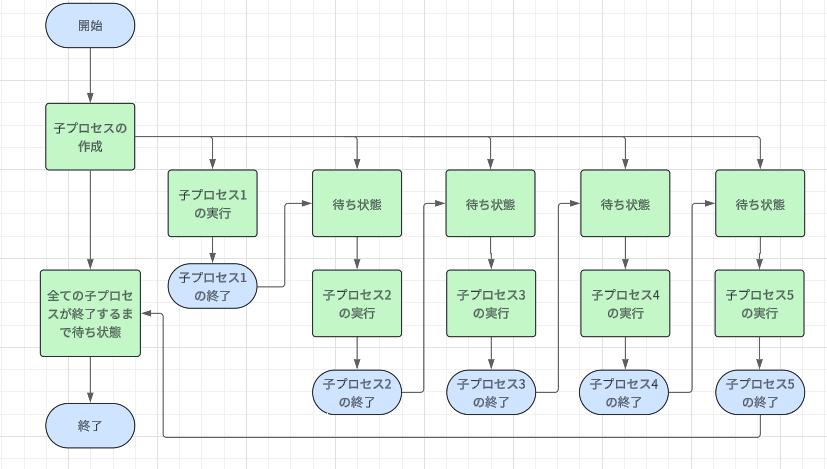
\includegraphics[width=12cm]{3-1hurotya.png}
    \caption{課題3-1の処理の流れ}
\end{figure}
\\
今回のfile-counterプログラムでは子プロセスを4つ作成し,それぞれの子プロセス内の処理を順番に一つずつ実行していく必要がある.
そのため,実行している子プロセス以外は待ち状態にしておき,実行中のプロセスが終了してから一つだけ待ち状態を開放して処理を実行するというアルゴリズムで今回の課題を実装した.フローチャートにおいて,子プロセスの終了から待ち状態へ伸びている矢印は
子プロセスが終わってから矢印の先の待ち状態が解放されるということを表している.今回の課題のクリティカルセクションは後述のcount1関数なので,この直前に待ち状態と解放を処理する関数を呼び出すようにした.
\subsection{実装方法}
ここではセマフォの処理について中心に記述する.以下は親プロセスのプログラムを抜粋したものである.
\begin{lstlisting}
if ((key = ftok(".", 1)) ==-1){
    fprintf(stderr,"ftok path does not exist.\n");
    exit(1);
}
//セマフォセットを作成
if ((sem_id=semget(key, 4, 0666 | IPC_CREAT)) ==-1) {
    perror("semget error.");
    exit(1);
}
// セマフォの初期値を1に設定
if (semctl(sem_id, 0, SETVAL, 1) == -1) {
    perror("semctl SETVAL error.");
    exit(1);
}
count = 0;

if ((ct=fopen(filename, "w"))==NULL) exit(1);
fprintf(ct, "%d\n", count);
fclose(ct);
for (i=0; i<NUMPROCS; i++) {
    if ((pid=fork())==-1) {
        perror("fork failed.");
        exit(1);
    }
    if (pid == 0) { 子プロセスの処理のため省略
    }
}
for (i=0; i<NUMPROCS; i++) {
wait(&status);
}

// セマフォを削除
if (semctl(sem_id, 0, IPC_RMID) == -1) {
    perror("semctl IPC_RMID error.");
    exit(1);
}
exit(0);
\end{lstlisting}
即ち,今回のプログラムにおける親プロセスの処理の流れは以下のようになる.
\begin{enumerate}
    \item セマフォセットの初期設定
    \item 子プロセスの作成
    \item 子プロセスがすべて終了するまで待つ
    \item セマフォの削除
\end{enumerate}
以下でその詳細について記述する.
\begin{enumerate}
    \item まず,ftok()を使ってkeyを作成する.このとき,第一引数の"."は現在のディレクトリを表し,第二引数の"1"はプロジェクトを一意に識別する文字を指定している.\cite{1}次にsemget()を使ってセマフォセットを作成している.
    第一引数は作成したkey,第二引数はセマフォの数である4,第三引数はアクセス許可の定義として使用され,全てに読み込み,書き込み許可を与えるという設定である.\cite{2}最後にsemctl()を使って0番目のセマフォの値を1に設定する.
    第一引数はセマフォIDのsem\_idを,第二引数でセマフォ番号の0を,第三引数のSETVALはsemvalの値を第四引数で指定された値に設定する制御操作を指定するパラメータ値である.セマフォの初期値を1に設定する理由については子プロセスの処理
    にて詳細を記述する.
    \item fork()を使って子プロセスを作成する.for文の中で呼び出すことによって子プロセスを複数作成する.fork()の返り値をpidに格納し,pidの値によって子プロセスを分岐させて親プロセスと子プロセスの処理内容を分ける.
    ここでは親プロセスについての記述なので,以下の3,4の記述は親プロセスの処理についてである.
    \item wait()を使って子プロセスの終了を待つ.引数には状況の情報値を格納する.2で作成したプロセスの数だけfor文でこれを繰り返すことですべてのプロセスが終了するまで待ち続けることができるようになる.\cite{3}
    \item 最後にセマフォをsemctl()を使って削除する.第三引数のIPC\_RMIDは第一引数によって指定されたセマフォIDをシステムから除去し,それに関連するセマフォセットを破棄する.\cite{2}
\end{enumerate}
また,子プロセスのプログラムは以下のようになる.
\begin{lstlisting}
if (pid == 0) { /* Child process */
    lock(sem_id);
    count = count1();
    printf("count = %d\n", count);
    unlock(sem_id);
    exit(0);
}
\end{lstlisting}
即ち,以下のような流れで処理が実行される.
\begin{enumerate}
    \item lock()の呼び出し
    \item count1()の呼び出し
    \item unlock()の呼び出し
    \item 子プロセスの終了
\end{enumerate}
以下でその詳細について記述する.
\begin{enumerate}
    \item pidの値が0のときは子プロセスであると判定できる.子プロセス内の処理がクリティカルセクションであるので,まずlock()を呼び出す.
    lock()のプログラムは以下のようになっている.
    \begin{lstlisting}
void lock(int semid){
    struct sembuf op;
    op.sem_num = 0;
    op.sem_op =-1;
    op.sem_flg = 0;
    if (semop(semid, &op, 1) == -1) {
        perror("semop lock");
        exit(1);
    }
}
    \end{lstlisting}
    ここではsemop()を使ってプロセスを停止している.第一引数はセマフォIDのsemid,第二引数はsembuf構造体のポインタ,第三引数は第二引数の数を表す.sembuf構造体は3津のメンバが存在し,sem\_numはセマフォ番号,sem\_opはセマフォ操作,sem\_flagは操作フラグを表す.\cite{4}sem\_opは-1,それ以外は0に指定することによって
    セマフォ値がsem\_opの値を足した結果0以上にならない場合はプロセスを停止する.セマフォ値の初期値を1にしていたことによって,最初のプロセスは停止しないが,次のプロセスはセマフォ値が0でsem\_opを加算すると負の値になってしまうので
    停止する.
    \item セマフォに関係する処理はないので省略する.
    \item unlock()のプログラムは以下の通りである.
    \begin{lstlisting}
void unlock(int semid){
    struct sembuf op;
    op.sem_num = 0; // セマフォの番号を固定値として指定
    op.sem_op = 1; // V操作(加算、アンロック)
    op.sem_flg = 0;
    if (semop(semid, &op, 1) == -1) {
        perror("semop V");
        exit(1);
    }
}
    \end{lstlisting}
    まずsemop()を使ってセマフォ値を変更し,子プロセスの待ち状態を一つ開放する.第二引数のsembuf構造体のsem\_opを1に,それ以外を0に設定することによって待っている一つの状態の子プロセスにおいて
    -1を加算してもセマフォ値が0以上になるので待ち状態ではなくなる.このようにして待ち状態のプロセスの開放を一つずつ行うことによってクリティカルセクションに複数のプロセスが同時にアクセスできないようにしている.
    \item exit()を使って子プロセスを終了する.
\end{enumerate}
\subsection{実行結果}
この実行結果は以下のようになる.
\begin{figure}[htbp]
    \begin{minipage}[b]{0.45\linewidth}
      \centering
      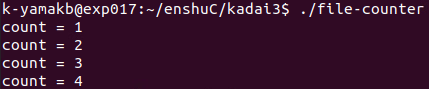
\includegraphics[keepaspectratio, scale=0.7]{result3-1.png}
      \caption{ターミナル上の実行結果}
    \end{minipage}
    \begin{minipage}[b]{0.45\linewidth}
      \centering
      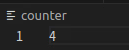
\includegraphics[keepaspectratio, scale=0.8]{result3-1-1.png}
      \caption{counterファイルの内容}
    \end{minipage}
  \end{figure}
  以上の結果により,きちんとcountが1ずつ増やされ,最終的にcounterファイルには4が記入されているということがわかる.


  \section{課題3-2-1}
\subsection{アルゴリズム}
この課題の処理の流れは以下図4のフローチャートのとおりである.
\begin{figure}[h]
    \centering
    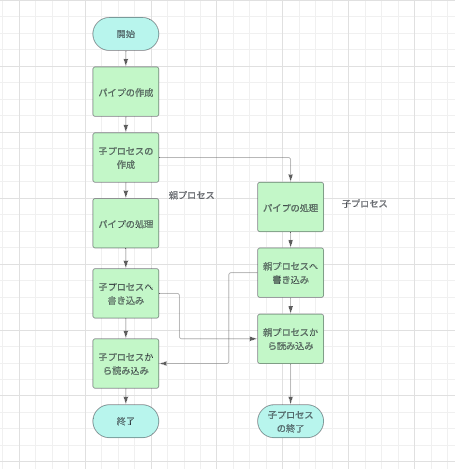
\includegraphics[width=6cm]{3-2hurotya.png}
    \caption{課題3-2の処理の流れ}
\end{figure}
\\
今回のtwo-way-pipeプログラムでは子プロセスを一つ作成し,子プロセスから親プロセスへ最初の引数の文字列を,親プロセスから子プロセスへ次の引数の文字列を送信する.
そして親プロセスは子プロセスから,子プロセスは親プロセスから送られてきた文字列を受け取り表示させる.図の左側は親プロセス,右側は子プロセスの処理を表す.
双方向のパイプを実現するために,子プロセス用のパイプと親プロセス用のパイプの二つのパイプを作成して実装した.
\subsection{実装方法}
パイプ部分を中心に実装方法を記述する.
記述する内容としては以下のとおりである.
\begin{enumerate}
    \item パイプの作成
    \item 子プロセスの処理
    \item 親プロセスの処理
\end{enumerate}
以下でその詳細について記述する.
\begin{enumerate}
    \item パイプの作成は,以下のようなプログラムになる.
    \begin{lstlisting}
if (pipe(parenttochild) == -1 || pipe(childtoparent) == -1) {
    perror("pipe failed.");
    exit(1);
}
    \end{lstlisting}
    pipe()を使い,親プロセスから子プロセスへ送信したり,親プロセスが読み込むためのパイプとしてparenttochild,子プロセスから親プロセスへ送信したり,子プロセスが読み込むためのパイプとしてchildtoparent
    を定義した.パイプを二つ作成した理由としては,パイプは安全のために書き込み側か読み込み側のどちらかをクローズする必要があるため,
    一つのパイプではどちらの機能も同時に使うことができないためである.
    \item fork()を使って子プロセスを一つ作成し,pidが0かどうかで親プロセスと子プロセスの処理を分離した.
    子プロセスのプログラムは以下の通りである.
    \begin{lstlisting}
    if (pid == 0) { /* Child process */
        close(parenttochild[1]);
        close(childtoparent[0]);
        msglen = strlen(argv[1]) + 1;
        if (write(childtoparent[1], argv[1], msglen) ==-1) {
            perror("pipe write.");
            exit(1);
        }
        if (read(parenttochild[0], buf, BUFSIZE) ==-1) {
            perror("pipe read.");
            exit(1);
        }
        printf("Message from parent process: %s\n",buf);
        wait(&status);
        exit(0);
    }
    \end{lstlisting}
    子プロセスではparenttochildの書き込み機能とchildtoparentの読み込み機能を使用しないので,まずこれらをclose()しておく.
    そして第二引数の文字列をwrite()を使って送信しread()を使って親プロセスから送られてきた第一引数の文字列を受信して標準出力に出力する.
    \item 親プロセスのプログラムは以下のとおりである.
    \begin{lstlisting}
    else { /* Parent process */
        close(parenttochild[0]);
        close(childtoparent[1]);
        msglen = strlen(argv[2]) + 1;
        if (write(parenttochild[1], argv[2], msglen) ==-1) {
            perror("pipe write.");
            exit(1);
        }
        if (read(childtoparent[0], buf, BUFSIZE) ==-1) {
            perror("pipe read.");
            exit(1);
        }
        printf("Message from child process: %s\n",buf);
        wait(&status);
    }
    \end{lstlisting}
    親プロセスではparenttochildの読み込み機能とchildtoparentの書き込み機能を使用しないのでこれらをclose()しておく.
    そして第一引数の文字列をwrite()を使って送信しread()を使って子プロセスから送られてきた第二引数の文字列を受信して標準出力に出力する.
\end{enumerate}
\subsection{実行結果}
以下はtwo-way-pipeプログラムを実行したときの結果である.
\begin{figure}[h]
    \centering
    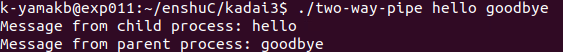
\includegraphics[width=10cm]{result3-2-1.png}
    \caption{two-way-pipe.cの実行結果}
\end{figure}
これにより,第一引数で与えられたhelloが子プロセスから,第二引数で与えられたgoodbyeが親プロセスから送られてきていることがわかる.
\section{課題3-2-2}
\subsection{アルゴリズム}
この課題の処理の流れは以下図6のフローチャートのとおりである.\clearpage
\begin{figure}[h]
    \centering
    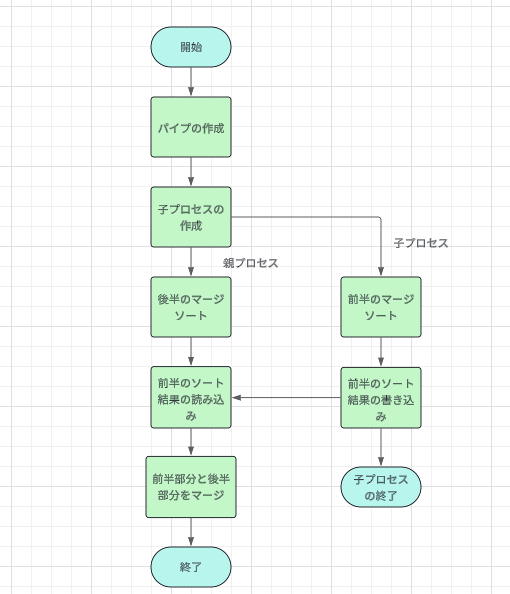
\includegraphics[width=8cm]{3-2-2hurotya.png}
    \caption{課題3-2の処理の流れ}
\end{figure}

今回のmergesortプログラムでは子プロセスを一つ作成し,子プロセスでソート対象の配列の前半半分を,親プロセスでソート対象の配列の後半半分をソートしてからマージするというアルゴリズムで作成した.
図6の左側が親プロセス,右側が子プロセスに対応する.また,子プロセスのソート結果を親プロセスに伝えるためにパイプを使用した.これにより前半と後半のソートを並列に実行できるようになる.
\subsection{実装方法}
ここではマージソートのアルゴリズムについては言及せず,どのようにして並列化をしたかについて中心に記述する.
今回,変更を加えたのはmergesort()内のみである.
関数mergesort中に図5のフローチャートの流れで並列化を実装したのでそれぞれの詳細について記述する.
\begin{enumerate}
    \item パイプの作成では,pipe()を使ってパイプfdを作成した.
    \item プロセスの作成では,fork()を使って子プロセスを作成し,pidが0かどうかで親プロセスと子プロセスの処理を分離した.
    子プロセスのプログラムは以下のようになる.
    \begin{lstlisting}
    if(pid == 0){/*child process*/
        close(fd[0]);
        m_sort(numbers, temp, 0, (array_size-1)/2);
        if (write(fd[1], numbers, ((array_size - 1) / 2 + 1) * sizeof(int)) ==-1) {
                perror("pipe write.");
                exit(1);
        }
        exit(0);
      }
    \end{lstlisting}
    子プロセスではfdの読み込み機能は使用しないので,まずclose()しておく.そして引数には0と配列の要素の中央値を渡してmsort()呼び出す.
    これによってソート対象の配列の前半部分をマージソートすることができる.次にwrite()を呼び出して前半がソートされた配列を親プロセスに送信する.このときに引数に0と配列の要素の中央値を渡すことで配列全体ではなく前半部分のみを送ることができる.
    配列全体を送ってしまうと親プロセスでソートされた部分と競合してしまい,正しいソート結果ではなくなってしまう.
    \item 親プロセスのプログラムは以下のようになる.
    \begin{lstlisting}
    else{/*parent pocess*/
        close(fd[1]);
        m_sort(numbers, temp, (array_size-1)/2+1, array_size - 1);
        if (read(fd[0], numbers, ((array_size - 1) / 2 + 1) * sizeof(int)) ==-1) {
            perror("pipe read.");
            exit(1);
        }
        merge(numbers, temp, 0, (array_size-1)/2+1, array_size-1);
    }
    \end{lstlisting}
    親プロセスではfdの書き込み機能は使用しないのでclose()しておく.親プロセスでは引数として配列の要素数の中央値と配列の要素数を渡してmsort()を呼び出す.これによってソート対象の配列の後半部分をマージソートすることができる.
    その後read()を使って子プロセスから送信された前半のソート結果を読み込む.このときに引数に配列の0と配列の要素数の中央値を渡すことで前半部分だけを読み込む.
    \item 最後に前半部分と後半部分をmergesort()を呼び出してソートする.
\end{enumerate}
\subsection{実行結果}
以下はmergesortを実行したときの結果である.
\begin{figure}[h]
    \centering
    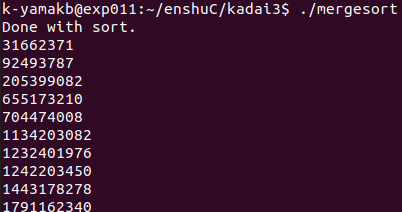
\includegraphics[width=6cm]{result3-2-2.png}
    \caption{mergesort.cの実行結果}
\end{figure}
このことから,昇順に正しくソートすることができていると考えられる.
\section{課題3-3-1}
\subsection{アルゴリズム}
この課題の処理の流れは以下図8のフローチャートの通りである.
\begin{figure}[h]
    \centering
    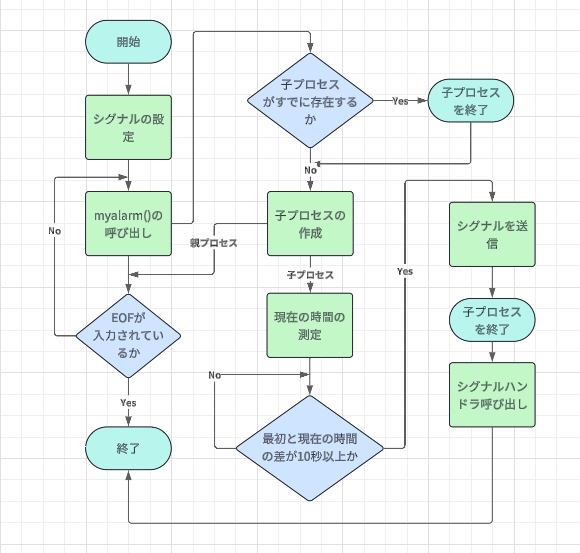
\includegraphics[width=8cm]{3-3-1.png}
    \caption{課題3-3-1の処理の流れ}
\end{figure}
\\
今回の課題ではalarmプログラム内のmyalarm()をalarm()を使用せずに実現するというものである.
alarm()は子プロセスが引数で指定した秒数secだけ経つとシグナルを送信し,親プロセス内でシグナルハンドラが呼び出される.
上図フローチャートの左部がmain()の処理,中央と右部がalarm()の処理を表している.
\subsection{実装方法}
今回の課題ではmyalarm()内の実装のみを求められているので,myalarm()の実装方法について詳細に記述する.
alarm()のプログラムは以下のようになる.
\begin{lstlisting}
void myalarm(int sec) {
    if (timer_pid > 0) {
        kill(timer_pid, SIGTERM); // 子プロセスを終了させる
        waitpid(timer_pid, NULL, 0); // 子プロセスの終了を待つ(ゾンビプロセス防止)
    }
    int pid;
    time_t start_time, current_time;
    int elapsed_seconds = 0;
    if ((pid=fork())==-1) {
        perror("fork failed.");
        exit(1);
    }
    if(pid==0){/*子プロセス*/
        time(&start_time);
        while (elapsed_seconds < sec) {
            time(&current_time);
            elapsed_seconds = difftime(current_time, start_time);
            sleep(1);
        }
        if (kill(getppid(),SIGALRM) ==-1) {
            perror("kill failed.");
            exit(1);
        }
        exit(0);
    }else{
        timer_pid = pid;
    }
}
\end{lstlisting}
以下ではその処理を順番に記述する.
\begin{enumerate}
    \item フローチャートから,myalarm()では最初にすでに子プロセスが存在しているかどうかを判定する.上のプログラムの2から5行目にこの処理を記述している.fork()の返り値をタイマー管理用のプロセスIDを格納しているグローバル変数timer\_pidに格納している.この変数は最初に-1に初期化されているので,myalarm()の呼び出しが初めてなのかどうかを子の変数の値によって判定することができる.
    まず最初にtime\_pidが正であるかどうかを判定している.fork()の返り値が格納されているので,正であれば子プロセスが存在する,つまり初めてのmyalarm()の呼び出しではないことがわかる.よって前回作成した子プロセスを終了させ,waitpid()を使って子プロセスの終了を待つことでゾンビプロセスが発生することを避ける.
    \item 次に子プロセスを作成する.時間経過を測定するためにfork()を使用し,pidによって条件分岐することで親プロセスと子プロセスの処理を分ける.25から27行目のように,親プロセスでは1で使用したtimer\_pidにfork()の返り値を格納する.
    \item 13から25行目のように,子プロセスではwhile文の繰り返しを一定時間が経過するまで繰り返し続けることで一定時間の計測を実現している.
    具体的には,myalarm()を呼び出したときの時刻とwhile文のそれぞれの繰り返し時の時刻との差を格納しているelapsed\_secondsと指定したsecを比較し,前者の方が大きくなった際にループを抜けるという処理としている.
    自刻の計測にはtime()を使用し,差の計算にはdifftime()を使用した.そしてループを抜けた後にkill()を使ってシグナルハンドラを起動するシグナルを送り,子プロセスを終了する.
\end{enumerate}
\subsection{実行結果}
以下はalarmプログラムを実行したときの結果である.
\begin{figure}[h]
    \centering
    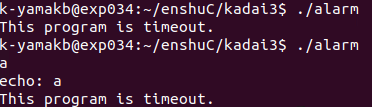
\includegraphics[width=8cm]{result3-3-1.png}
    \caption{alarmの実行結果}
\end{figure}
一回目の実行では何も入力せずにしばらく待った.このとき,タイムアウトの文字列が表示されてプログラムが終了した.また,二回目の実行ではプログラムを実行してから5秒たってから文字列aを入力してからしばらく待った.
このとき,aを入力してから10秒後にプログラムが終了した.以上のことから,プログラムが仕様通りに動作していることがわかる.
\section{課題3-3-2}
\subsection{アルゴリズム}
この課題の処理の流れは以下のフローチャートの通りである.
\begin{figure}[h]
    \centering
    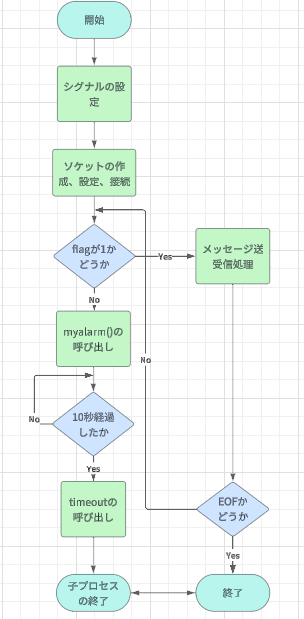
\includegraphics[width=7cm]{3-3-2.png}
    \caption{課題3-3-2の処理の流れ}
\end{figure}
\\この課題は大部分が課題2の内容なので,以下では追加した点について中心に記述する.図5のmyalart()の呼び出しの下側は子プロセスの処理,右側は親プロセスの処理となっている.
また,それぞれのプロセスの終了から出ている両方向への有向辺は一方のプロセスが終了するともう一方のプロセスの処理も終了するということを示している.
これによって,10秒間経過するかEOFが入力されたときにどちらのプロセスも終了させることができる.
\subsection{実装方法}
以下では4で述べたmyalarm()を使用するので,この関数については詳細を記述しない.
上のフローチャートより,このプログラムが処理する内容は以下のとおりである.
\begin{enumerate}
    \item シグナル,ソケットの設定
    \item 繰り返し文の処理
    \item シグナルハンドラtimeoutの設定
    \item タイムアウトの条件分岐
\end{enumerate}
以下でその詳細について述べる.
\begin{enumerate}
    \item シグナルとソケットの設定は課題3-3-1,課題2と同様に,以下のプログラムのように設定した.
    \begin{lstlisting}
    if(signal(SIGALRM,timeout) == SIG_ERR) {
        perror("signal failed.");
        close(sock);
        exit(1);
    } 
    if ((sock = socket(AF_INET, SOCK_STREAM, IPPROTO_TCP)) < 0) {
        perror("socket");
        exit(1);
    }

    /* ホストが存在するか確認 */
    server = gethostbyname(argv[1]);
    if (server == NULL) {
        fprintf(stderr, "ERROR, no such host as %s\n", argv[1]);
        exit(0);
    }

    /* ソケットアドレス再利用の指定 */
    reuse = 1;
    if (setsockopt(sock, SOL_SOCKET, SO_REUSEADDR, &reuse, sizeof(reuse)) < 0) {
        perror("setsockopt");
        exit(1);
    }
    /*サーバ受付用アドレスの設定*/
    bzero((char *)&svr, sizeof(svr));
    svr.sin_family = AF_INET;
    bcopy((char *)server->h_addr, (char *)&svr.sin_addr.s_addr, server->h_length);
    svr.sin_port = htons(10130);

    /* ソケットをサーバに接続 */
    if (connect(sock, (struct sockaddr *)&svr, sizeof(svr)) < 0) {
        perror("client: connect");
        close(sock);
        exit(1);
    }
    printf("connected\n");
    \end{lstlisting}
    \item 繰り返し文のプログラムは以下のようになる.
    \begin{lstlisting}
    do {
        myalarm(TIMEOUT);
        /* 入力を監視するファイル記述子の集合を変数rfdsにセットする */
        FD_ZERO(&rfds);
        FD_SET(0, &rfds); /* 標準入力 */
        FD_SET(sock, &rfds); /* ソケット */
        /* 監視する待ち時間を10秒に設定 */
        tv.tv_sec = 15;
        tv.tv_usec = 0;
        /* 標準入力とソケットからの受信を同時に監視する */
        if (select(sock + 1, &rfds, NULL, NULL, &tv) > 0) {
            if (FD_ISSET(0, &rfds)) {
                bzero(rbuf, 1024);
                if (fgets(rbuf, 1024, stdin) == NULL) {
                    if (timer_pid > 0) {
                        kill(timer_pid, SIGTERM); // 子プロセスを終了させる
                        waitpid(timer_pid, NULL, 0); // 子プロセスの終了を待つ(ゾンビプロセス防止)
                    }
                    printf("\nEOF detected\n");
                    break;
                }
                n = write(sock, rbuf, strlen(rbuf));
                if (n < 0) {
                    perror("ERROR writing");
                    break;
                }
            }
            if (FD_ISSET(sock, &rfds)) {
                bzero(rbuf, 1024);
                n = read(sock, rbuf, 1024);
                if(n <= 0){
                    perror("Connection closed by client.\n");
                    close(sock);
                    return 0;
                }else{
                    printf("%s",rbuf);
                }
            }
        }
    } while (!flag);
    \end{lstlisting}
    ここでは大きく分けて以下のような処理が繰り返し実行されている.
    \begin{enumerate}
        \item myalarm()の実行
        \item select()による待ち状態
    \end{enumerate}
    以下でこれらについて詳細に記述する.
    \begin{enumerate}
        \item select()による待ち状態は基本的には前回の課題の内容なので記述しないが,EOFを入力した際の処理には変更を加えたのでそれについて記述する.EOFを入力すると親プロセスが繰り返し文からbreakし,プログラムが終了するが
        alarm()を呼び出した後だと親プロセスが終了してから子プロセスが終了するので演習室環境が落ちてしまうことがあった.したがって,繰り返し文から出る前の15から18行目に課題3-3-1のゾンビプロセスをなくす処理と同じ以下のプログラムをつけることで
        この問題を解決した.
        \item alarm()は一度呼び出されてから10秒以内にもう一度呼び出すと前回呼び出した際のプロセスを終了する.これによって,何も入力されない状態が10秒続けば
        シグナルが送信されプログラムが終了するという機能が達成される.
        また,この繰り返し文の繰り返し条件は初期値が0のグローバル変数flagが1でないときである.この変数の処理についてはシグナルハンドラにおいて詳細に記述する.
    \end{enumerate}
    \item シグナルハンドラtimeout()のプログラムは以下のようになる.
    \begin{lstlisting}
    void timeout(){
        flag = 1;
    }
    \end{lstlisting}
    シグナルハンドラは仕様により非同期安全な関数のみしか使用できない.したがって,printfのような関数は使用できないため,今回のプログラムではシグナルハンドラtimeout内では
    flagという変数の値を変更するだけとした.このflagは子プロセス内で10秒が経過したときに1となり,それ以外は0のグローバル変数である.これによって先ほどの繰り返し文の条件が変更されるので10秒たった時点で親プロセスは
    繰り返しから抜けることができるようになる.
    \item タイムアウトが発生すると先ほどシグナルハンドラで立てたflagが1となる.それによって繰り返し文から抜けた後以下のプログラムが実行される.
    \begin{lstlisting}
        if(flag == 1){
        printf("This program is timeout.\n");
    }
    close(sock);
    return 0;
    \end{lstlisting}
\end{enumerate}
これによってタイムアウトしてプログラムが終了したことが表示される.
\subsection{実行結果}
以下はexp029というホスト名でsimple-talk-clientを,exp001というホスト名でsimple-talk-serverを実行したときの結果である.
\begin{figure}[htbp]
    \begin{minipage}[b]{0.45\linewidth}
      \centering
      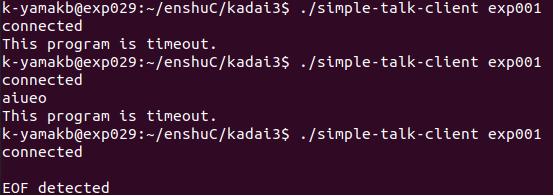
\includegraphics[keepaspectratio, scale=0.5]{result3-3-2-1.png}
      \caption{ターミナル上の実行結果}
    \end{minipage}
    \begin{minipage}[b]{0.45\linewidth}
      \centering
      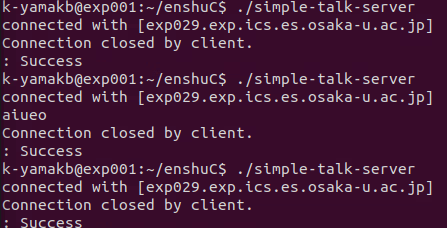
\includegraphics[keepaspectratio, scale=0.5]{result3-3-2-2.png}
      \caption{counterファイルの内容}
    \end{minipage}
  \end{figure}
上の結果では,以下の三通りの方法でプログラムを実行している.
\begin{enumerate}
    \item 何も入力せずに待ち続ける.
    \item 約5秒たってから文字列aiueoを送信して待ち続ける.
    \item EOFを入力する.
\end{enumerate}
以下でその実行結果について詳細を述べる.
\begin{enumerate}
    \item 何もせずに待ち続けるとmyalarm()で作成された子プロセスによってシグナルが送信され,シグナルハンドラが呼び出されてフラグの情報が変更される.これによってプログラムが終了するとともにタイムアウトした
    という文字列が表示されている.
    \item aiueoという文字列を入力しても前回の課題のようにメッセージを送受信することができていることがわかる.また,メッセージを送信してから10秒後にプログラムが終了したことから,使用を満たしていることがわかる.
    \item EOFを入力しても正常にプログラムが終了していることがわかる.
\end{enumerate}
\section{発展課題2}
\subsection{アルゴリズム}
今回の課題では課題3-2-2における,子プロセスによるマージソート高速化プログラムを改良し,指定された任意のk個のプロセスに
配列を分解してソートするプログラムを作成した.
この課題ではmergesort()の部分のみを変更したのでその部分のフローチャートを以下に示す.
\begin{figure}[h]
    \centering
    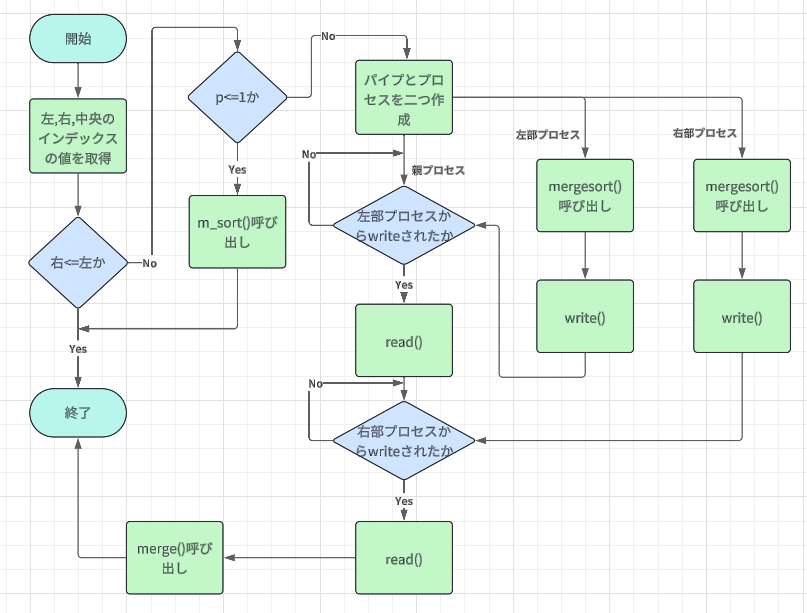
\includegraphics[width=8cm]{hatten2hurotya.png}
    \caption{mergesort()のフローチャート}
\end{figure}
フローチャート中のpは,そのプロセスにおいて作成しなければならないプロセスの個数を表す.\\
このプログラムでは任意のk個のプロセスに分解する方法として二分木の形状で再帰的にmergesort()を呼び出すという方法を採用した.具体的には,以下の手順に従っている.
\begin{enumerate}
    \item 配列を右部と左部に分け,それぞれに対応する子プロセスを作成する.以下ではこれらをそれぞれ左部のプロセス1.1と右部のプロセス1.2と呼ぶ.各プロセスの数字は二分木におけるの深さと左から何番目であるかに対応するものとする.
    このとき,子プロセスを作成してmergesort()を呼び出すがその際のpは左部のプロセスでは$p_left=\frac{p}{2}$,右部のプロセスでは$p_right=p-p_left$として引数にする.
    \item さらにプロセス1.1を左部のプロセス2.1と右部のプロセス2.2に分ける.右プロセスも同様に分ける.
    \item 合計の子プロセスの個数が指定したkに達するまで行う.kに達したかどうかは引数として与えているpの値が子プロセスになるにつれて減少していることから判断する.
\end{enumerate}
実際に9個のプロセスに分けると考えたときの二分木の様子は以下のようになる.\clearpage
\begin{figure}[h]
    \centering
    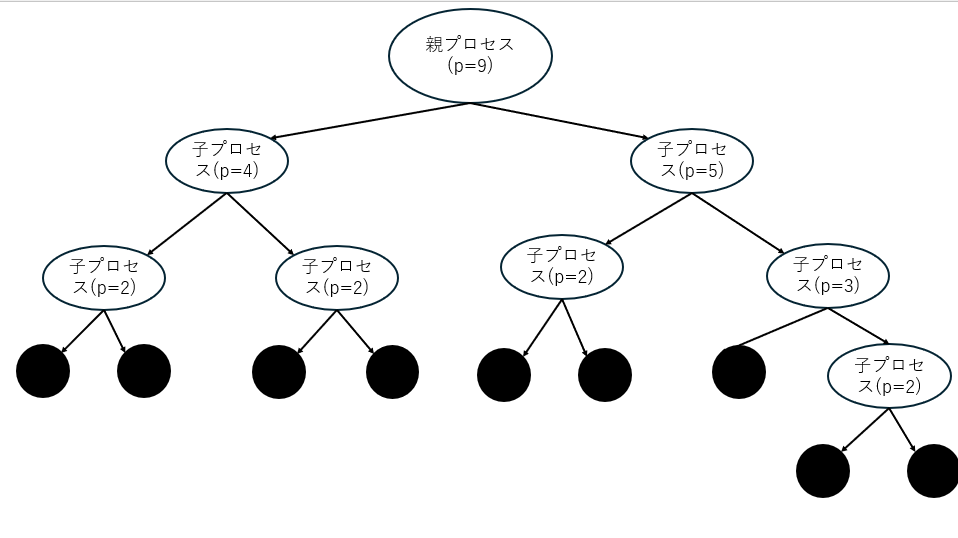
\includegraphics[width=8cm]{hatten2tree.png}
    \caption{実際にプロセスに分ける様子}
\end{figure}
黒い葉はp=1のときの子プロセスを表しており,それぞれの白い節点で葉の処理が終わってからmerge()が呼び出される.

\subsection{実装方法}
mergesort()の引数は以下のようになっている.
\begin{lstlisting}
    void mergeSort(int numbers[], int temp[], int left, int right, int p);
\end{lstlisting}
numbersとtempは課題3-2-2と同じで,ソートする対象の左端と右端を表すleftとright,そのプロセスにおいて作成しなければならないプロセスの個数であるpを引数として追加した.
先ほどのアルゴリズムで示したように,mergesort()を再帰的に呼び出す処理を行う.そのための処理としては以下のプログラムのようになる.
\begin{lstlisting}
if (left_pid == 0) {
    close(fd_left[0]);
    mergeSort(numbers, temp, left, mid, p_left);
    if (write(fd_left[1], &numbers[left], size_left * sizeof(int)) == -1) {
        perror("pipe write.");
        exit(1);
    }
    close(fd_left[1]);
    exit(0);
}
\end{lstlisting}
上は左部プロセスについての処理である.再帰的に呼び出すために,mergesort()の引数として左端をleft,右端を$mid = \frac{left+right}{2}$とした.
\begin{lstlisting}
if (right_pid == 0) {
    close(fd_right[0]);
    mergeSort(numbers, temp, mid + 1, right, p_right);
    if (write(fd_right[1], &numbers[mid + 1], size_right * sizeof(int)) == -1) {
        perror("pipe write.");
        exit(1);
    }
    close(fd_right[1]);
    exit(0);
}
\end{lstlisting}
また,右部プロセスについての処理である.再帰的に呼び出すために,mergesort()の引数として左端をmid+1,右端をrightとした.パイプの処理についてはどちらのプロセスでも書き込みをしたいので二つのパイプfd\_leftとfd\_right
を使用した.そして左部プロセスと右部プロセスの両方が終了すればそのプロセスにおけるleft,mid,rightを使ってmerge()を実行する.
\subsection{実行結果}
以下はhatten2.cの実行結果である.
\begin{figure}[h]
    \centering
    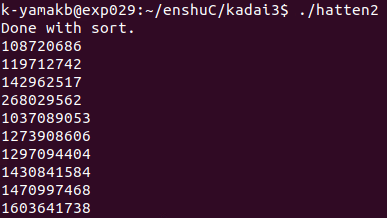
\includegraphics[width=8cm]{resulthatten2.png}
    \caption{発展課題2の実行結果}
\end{figure}
\\このことから,正しく昇順にソートすることができていることがわかる.課題3-2-2との比較については考察にて詳細を述べる.
\section{発展課題3}
\subsection{アルゴリズム}
ここでは交互実行をセマフォを使って実装した.具体的な処理の流れは以下のフローチャートのようになる.
\begin{figure}[h]
    \centering
    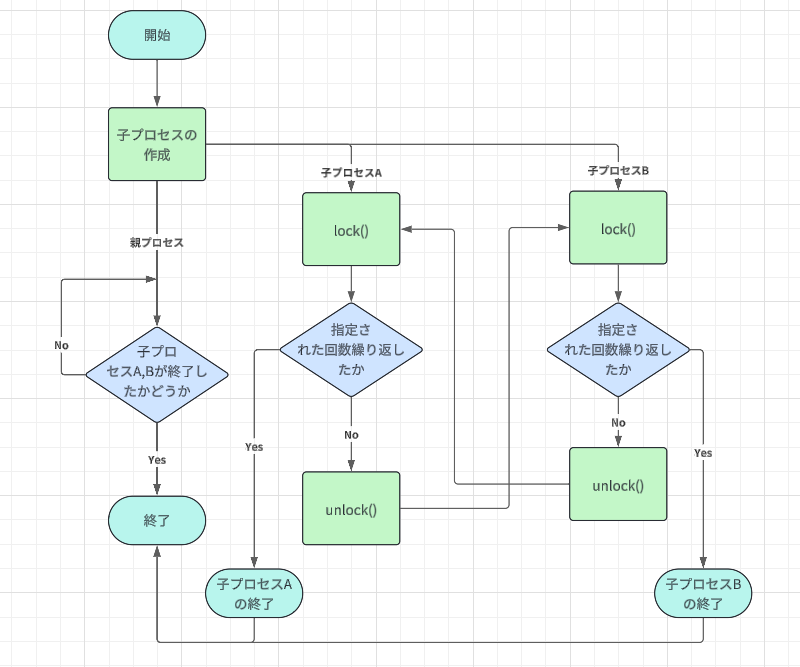
\includegraphics[width=8cm]{hatten3hurotya.png}
    \caption{発展課題3のフローチャート}
\end{figure}
\\ここで登場するlock()とunlock()は課題3-1で使用したものと同じである.unlock()からlock()に有向辺が出ているのは,セマフォの値をunlock()で増加させることで,lock()により待ち状態であったもう一方の子プロセスを開放するということを表す.
これにより,お互いに待ち状態と実行状態を交互に繰り返すようにした.
\subsection{実装方法}
実装方法としては,以下のとおりである.
\begin{enumerate}
    \item セマフォ用のキーを作成し,セマフォセットを作成して初期値を1とする.
    \item 子プロセスを二つ作成する.子プロセスAではグローバル変数の配列A\_listを要素数だけ標準出力に出力する.子プロセスBではグローバル変数の配列B\_listを要素数だけ標準出力に出力する.
    \item 親プロセスでは子プロセスの終了を待ち,両方のプロセスが終了すればセマフォを開放する.
\end{enumerate}
いかに詳細を記述する.
\begin{enumerate}
    \item ここは課題3-1と同様なので省略する.
    \item 子プロセスAの処理は以下のようなプログラムである.
    \begin{lstlisting}
        if (a_pid == 0) { // 子プロセスA
        for (int i = 0; i < NUM; i++) {
            lock(sem_id);
            printf("a%d\n", A_list[i]);
            unlock(sem_id);
        }
        exit(0);
    }
    \end{lstlisting}
    NUMには配列A\_listとB\_listの要素数を表す変数が格納されており,printf()が呼ばれるたびにlock()とunlock()が上のようなタイミングで呼び出される.
    これは課題3-1の時と同様にセマフォの値がunlock()を呼び出すたびに1増加されてもう一方のプロセスで待ち状態が解放されて処理が始まるということを表し,これにより交互に実行することが実現される.
    \\
    また,子プロセスBの処理は以下のようなプログラムである.
    \begin{lstlisting}
        if (b_pid == 0) { // 子プロセスB
        for (int i = 0; i < NUM; i++) {
            lock(sem_id);
            printf("b%d\n", B_list[i]);
            unlock(sem_id);
        }
        exit(0);
    }
    \end{lstlisting}
    これも子プロセスAと同様である.
    \item プロセスの待ちとセマフォの開放は以下のようになる.
    \begin{lstlisting}
    wait(NULL);
    wait(NULL);

    // セマフォを解放
    if (semctl(sem_id, 0, IPC_RMID) == -1) {
        perror("semctl IPC_RMID エラー.");
        exit(1);
    }
    \end{lstlisting}
\end{enumerate}
\subsection{実行結果}
以下はhatten3.cの実行結果である.
\begin{figure}[h]
    \centering
    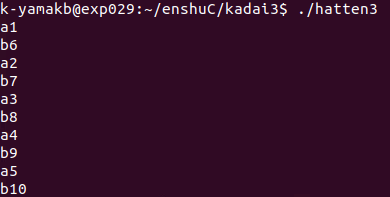
\includegraphics[width=8cm]{resulthatten3.png}
    \caption{発展課題3の実行結果}
\end{figure}
\\このことから子プロセスAと子プロセスBの処理を交互に実行することができていることがわかる.
\section{考察と感想}
今回の課題を通して私が考察したのは,発展課題2でも述べた通り課題3-2-2と発展課題2の実行時間の比較である.これらのプログラムの実行時間を比較するために
以下のプログラムによって時間の平均を測定した.
\begin{lstlisting}
#include <stdio.h>
#include <stdlib.h>
#include <time.h>

#define NUM_TRIALS 100

double get_execution_time(const char* command) {
    clock_t start, end;
    start = clock();
    system(command);
    end = clock();
    return ((double)(end - start)) / CLOCKS_PER_SEC;
}

int main() {
    double total_time_h2c = 0.0;
    double total_time_mc = 0.0;
    double times_h2c[NUM_TRIALS];
    double times_mc[NUM_TRIALS];

    for (int trial = 0; trial < NUM_TRIALS; trial++) {
        times_h2c[trial] = get_execution_time("./h2c");
        total_time_h2c += times_h2c[trial];
        times_mc[trial] = get_execution_time("./mc");
        total_time_mc += times_mc[trial];
    }

    double mean_time_h2c = total_time_h2c / NUM_TRIALS;
    double mean_time_mc = total_time_mc / NUM_TRIALS;

    double variance_h2c = 0.0;
    double variance_mc = 0.0;

    for (int trial = 0; trial < NUM_TRIALS; trial++) {
        variance_h2c += (times_h2c[trial] - mean_time_h2c) * (times_h2c[trial] - mean_time_h2c);
        variance_mc += (times_mc[trial] - mean_time_mc) * (times_mc[trial] - mean_time_mc);
    }

    variance_h2c /= NUM_TRIALS;
    variance_mc /= NUM_TRIALS;

    printf("Average execution time for h2c: %e seconds\n", mean_time_h2c);
    printf("Variance of execution time for h2c: %e seconds^2\n", variance_h2c);
    printf("Average execution time for mc: %e seconds\n", mean_time_mc);
    printf("Variance of execution time for mc: %e seconds^2\n", variance_mc);

    return 0;
}
    
\end{lstlisting}
このプログラムはh2cとmcをそれぞれ100回ずつ実行しそれらの平均と分散を計算して表示するプログラムである.h2cは発展課題2,mcは課題3-3-2の実行ファイルである.計算時間が短いので指数型表示にするようにした.
また,ソートする対象の配列の要素数は10000個に設定した.
また,これらのプログラムの実行はどちらも演習室環境で行った.
以下はそれぞれプロセス数を変えて実行したときの結果である.
\begin{figure}[htbp]
    \begin{minipage}[b]{0.45\linewidth}
      \centering
      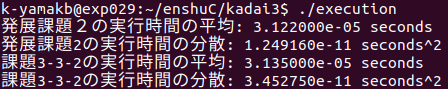
\includegraphics[keepaspectratio, scale=0.5]{resultproc2.png}
      \caption{プロセス数が2の時の実行時間}
    \end{minipage}
    \begin{minipage}[b]{0.45\linewidth}
      \centering
      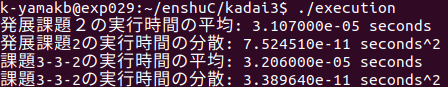
\includegraphics[keepaspectratio, scale=0.5]{resultproc3.png}
      \caption{プロセス数が3の時の実行時間}
    \end{minipage}
  \end{figure}
\\このようにして様々なプロセス数に対してプログラムを実行して実行時間の比較をしたが,あまり顕著な比較をすることができなかった.
それぞれの平均の差が$10^{-6}$程度の差しかなかったので,一つ一つのプログラムの処理がもう少し時間のかかるものでないと比較するのは難しいのではないかと感じた.
配列の要素数を増やして実行時間を上げようとしたが100000個にして処理時間を上げようと試みたが,演習室環境だと結果が出てこなかったので実行できなかった.
これは.グローバル変数として定義する配列はメモリに格納されるが,その要素数が大きいとメモリ確保に失敗することが原因であると考えた.
このことから,今回の発展課題のプログラムでは具体的にどれほどの改善ができたかを可視化することはできなかった.夏休みなどの時間があるときに
またほかの手法などについて考えたり調べたりしてみたいと思う.
\section{謝辞}
今回の課題にあたって質問対応やレポート採点をしていただいた教授及びTAの皆様,ありがとうございました.課題4も引き続きよろしくお願い致します.
\begin{thebibliography}{99}
    \bibitem{1} \url{https://www.ibm.com/docs/ja/aix/7.3?topic=f-ftok-subroutine} 6/12アクセス
    \bibitem{2} \url{https://www.ibm.com/docs/ja/aix/7.3?topic=s-semget-subroutine} 6/12アクセス
    \bibitem{3} \url{https://www.ibm.com/docs/ja/zos/2.5.0?topic=functions-wait-wait-child-process-end} 6/12アクセス
    \bibitem{4} \url{https://www.c-lang.net/semop/index.html} 6/12アクセス
\end{thebibliography}
\end{document}